\section{Approach}
\label{sec:approach}

\subsection{Overview}

\sys takes two inputs: a working source program, and a set of requirements that state which properties the clone must change (e.g., ``replace the TLS library with a memory-safe alternative,'' ``prefer faster numerical routines,'' or ``obscure the proprietary estimation logic''). It produces a clone: a program that reproduces the observable behavior of the original while differing from it in the intended ways. Figure~\ref{fig:architecture} presents the architecture.

\begin{figure*}[t]
\centering
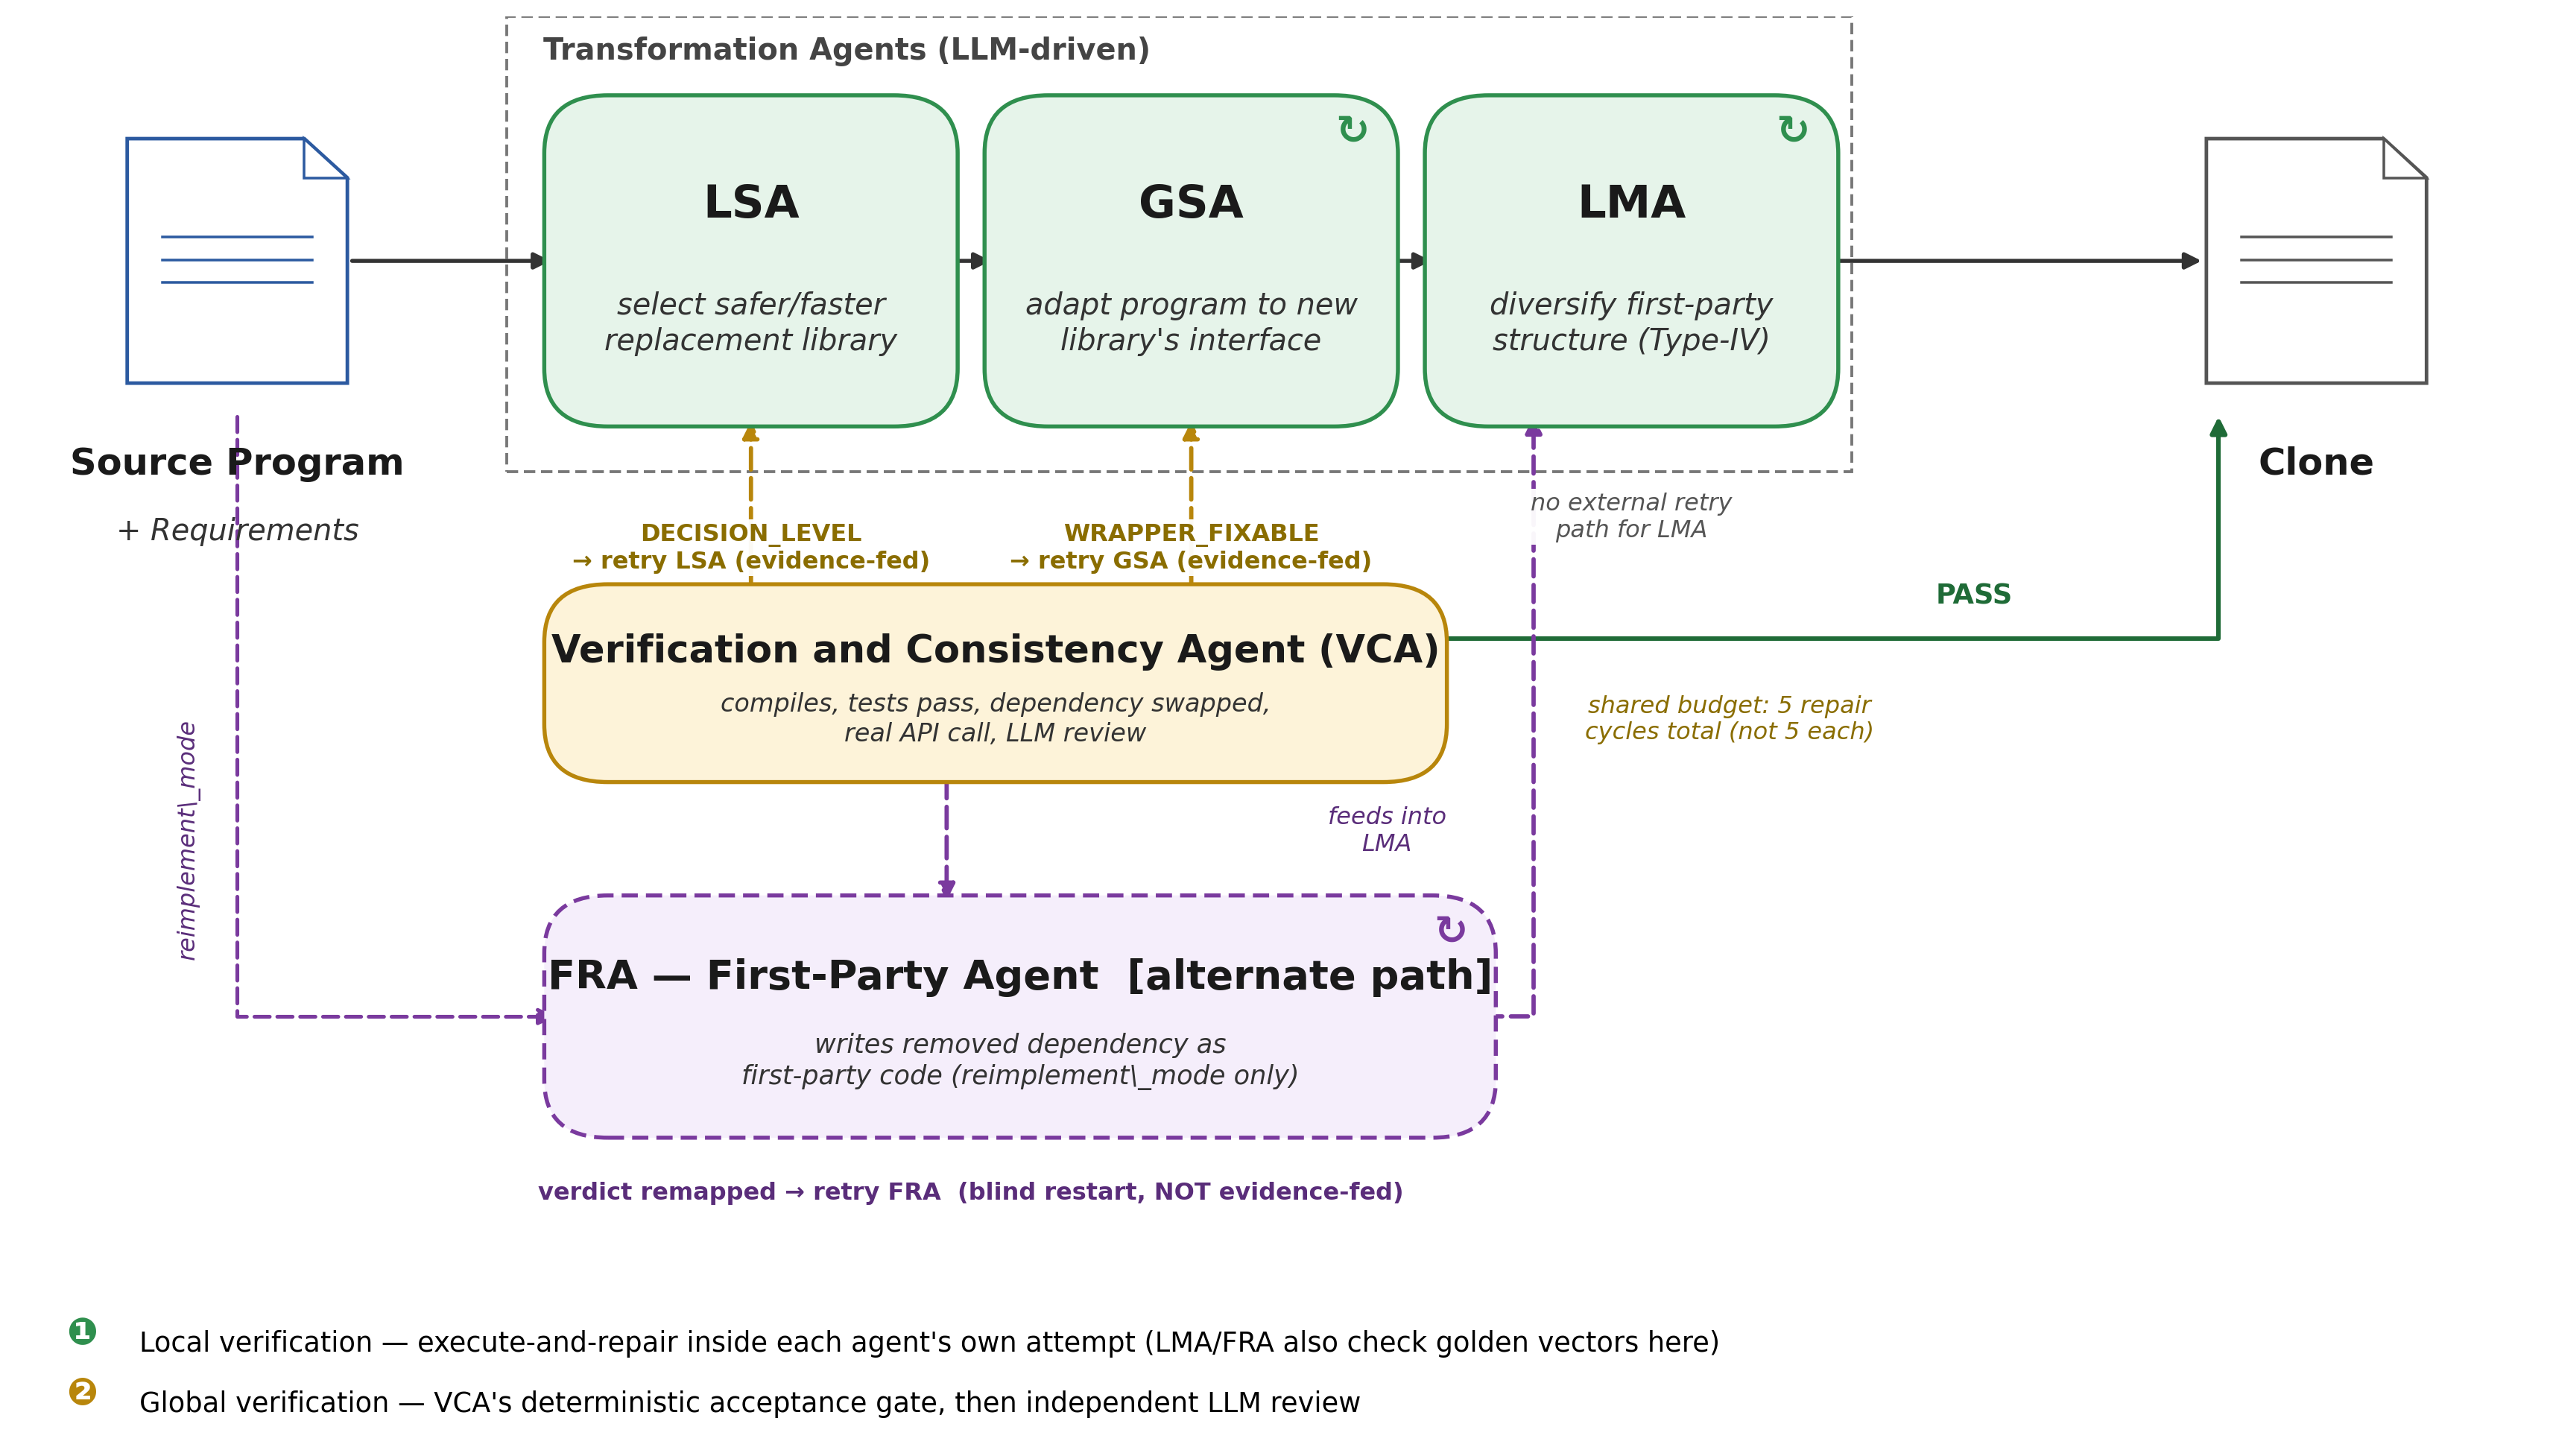
\includegraphics[width=0.92\linewidth]{figs/architecture_overview.png}
\caption{\sys's architecture. The default path routes a source program through the Library-Substitution Agent (LSA), Glue-Synthesis Agent (GSA) and Logic-Mutation Agent (LMA) in sequence; the First-Party Agent (FRA) replaces the LSA/GSA pair on the alternate path taken when no library exists to substitute, and feeds into the same LMA every path shares. The Verification and Consistency Agent (VCA) gates every candidate against a deterministic migration-completeness check and an independent model review, and routes each failure to the specific agent responsible for it, drawn from one shared budget of five repair cycles per run; the LMA is never itself a re-entry target, by construction. Section~\ref{sec:looping} details exactly which retries are evidence-fed and which are not.}
\label{fig:architecture}
\end{figure*}

The transformation is not performed in a single pass, and it is not performed by four agents alone. \sys first routes the program through a deterministic, non-LLM \emph{evidence-gathering front end} (a Parser that extracts every import and call site, and a Security stage that checks each incumbent dependency against known vulnerabilities) before any model call is made. An LLM-driven Resolver then proposes candidate replacement libraries, a second Security pass vets those candidates specifically, and a Profiler benchmarks their import cost and runtime performance, all before the \emph{Library-Substitution Agent} (\emph{LSA}) scores and selects among them. Only once a target is chosen does the pipeline move to the \emph{Glue-Synthesis Agent} (\emph{GSA}), which reconciles the program with the new interface, then to the \emph{Logic-Mutation Agent} (\emph{LMA}), which diversifies first-party structure, and finally to the \emph{Verification and Consistency Agent} (\emph{VCA}), which is the sole authority for whether the pipeline advances, loops back, or stops. An optional human approval gate can sit between the LSA's decision and any file write; a fifth agent, the \emph{First-Party Agent}, can stand in for the LSA and GSA together when the requirement is not ``swap library A for library B'' but ``remove the dependency and reimplement its behavior as first-party code.''

The key design principle is separation of concerns under verification: every agent mutates only the code (or, for the front-end stages, only the evidence) it is responsible for, and no agent's output advances to the next stage until it has been shown to execute correctly. The core engine of each LLM-driven agent is a model prompted with the current program state, the agent's specific objective, and, crucially, the concrete evidence (errors, test results, benchmark numbers, vulnerability reports) available at that point in the pipeline.

\subsection{Evidence-Gathering Front End}
\label{sec:frontend}

Three of the pipeline's stages run before any transformation decision is made, and two of the three involve no LLM call at all.

\textbf{Parser.} A deterministic AST walk over the source file. It extracts every import statement and, for each imported package, records which of its API methods are actually called at which call sites: context the Resolver and later agents consume but do not have to re-derive themselves.

\textbf{Security (incumbent, then candidates).} Each currently-imported third-party package is checked against public vulnerability and package-freshness signals (advisory count, release recency, yanked-version status), skipping first-party modules. The same check runs a second time, later in the pipeline, against the specific candidate replacement packages the Resolver proposes, since these were not import statements in the original file and are otherwise invisible to the first pass. Both passes are deterministic lookups, not LLM calls; their output is a vulnerability/freshness score the LSA's decision step penalizes incumbents and candidates by.

\textbf{Profiler.} Benchmarks each candidate package's import cost and the runtime performance of its relevant API calls, via repeated subprocess measurement in an isolated environment. Also deterministic; its output feeds the same scoring step as Security's.

These three stages exist so that the LSA's decision is grounded in measured evidence (vulnerability status, benchmark numbers) rather than the model's prior beliefs about which library is ``better.''

\subsection{The Transformation Agents}

\textbf{1. Library-Substitution Agent (LSA).} The LSA is responsible for selecting among third-party dependencies. It is realized as two cooperating steps: a \emph{Resolver} call that groups candidate libraries into equivalence classes (clusters of packages that could plausibly substitute for a given role, discovered independently of what the file currently imports), and a \emph{scoring and decision} call that combines the Security stage's vulnerability signal and the Profiler's performance numbers into a weighted choice per equivalence group. The LSA records the interface delta, the functions, types, and invariants that differ between the incumbent and the substitute, for downstream agents to act on; it does not itself rewrite the surrounding program. When a substitution has been selected, the pipeline proceeds to the GSA; when the LSA's own scoring flags that the winning candidate's API is not a close-enough match, or that a candidate explicitly requires glue, the same routing sends the program to the GSA as well, so the GSA is entered only when it is actually needed and skipped for genuine drop-in replacements.

\textbf{2. Glue-Synthesis Agent (GSA).} Substituting a dependency is rarely a drop-in replacement: signatures differ, initialization differs, and error-handling conventions differ. The GSA synthesizes the glue code (adapters, shims, and initialization logic) that reconciles the program with the substitute's interface, using the interface delta the LSA produced. It operates directly on the real file through an agent-computer interface (ACI) editing session (Section~\ref{sec:impl}) rather than regenerating the module wholesale, so an unrelated part of the file is never touched. The GSA makes the new dependency fit without disturbing the application logic that consumes it; it does not decide \emph{which} logic that is or restructure it, which is the LMA's job.

\textbf{3. Logic-Mutation Agent (LMA).} The LMA targets first-party structure, and it runs regardless of whether a library substitution occurred: it is the same tail stage whether the program arrived via the LSA/GSA path or via the First-Party Agent (Section~\ref{sec:fra}) below. Rather than bridging behavioral differences between an old and new library (that is the GSA's or the First-Party Agent's job, and their output has already been shown to execute correctly by the time the LMA sees it), the LMA further diversifies the already-working program's structure: it may restructure control flow, re-express algorithms, rename and re-decompose functions, and alter data representations, while an oracle gates every candidate so only behavior-preserving rewrites survive. It searches for a rewrite at an approximately requested size using a beam-search procedure adapted from Auto-SPT~\cite{hooda2025autospt}, with the clone-detector objective that work optimizes replaced by a size objective, since \sys's goal is behavioral equivalence at a target degree of structural divergence rather than evasion of a specific detector. We deliberately exclude third-party library code from the LMA's scope: mutating a well-tested library's internals introduces risk without benefit, whereas mutating first-party logic is precisely what yields a Type~IV clone of the code that matters.

\textbf{4. Verification and Consistency Agent (VCA).} The VCA does not mutate code; it interrogates it, and it is the only agent that decides whether the pipeline advances, retries, or stops. It runs in two stages. The first is deterministic: static analysis (a linter, a security-focused static checker, and a type checker, plus an import smoke test), a check that the subject's own test suite still passes against the patched code, and a migration-completeness gate asking three questions no project test answers directly: is the source library genuinely gone, is the target library actually called rather than merely imported, and does one real, uninjected call into the program's own API misuse it. That gate deliberately never consults a golden vector or a recorded invariant, even though the Logic-Mutation and First-Party Agents already check exactly that evidence in their own local loop (Section~\ref{sec:looping}): an acceptance gate handed the same answer key the scoring oracle uses would not be an independent check. All of this produces findings with no LLM tokens spent. The second is an LLM review that reads those findings alongside the GSA's own self-reported assessment of what it did and did not resolve, and renders one of three verdicts per candidate: \textsc{pass} (advance); \textsc{wrapper\_fixable} (a bug in the adapter that the GSA can plausibly repair given the concrete error, so the pipeline re-enters the GSA); or \textsc{decision\_level} (the selected library itself cannot satisfy the requirement no matter how the glue is written, so the pipeline re-enters the LSA with that candidate excluded from consideration). This routes each failure to the agent actually responsible for it rather than restarting the whole pipeline, and is explicitly a Reflexion-style~\cite{shinn2023reflexion} self-correction discipline rather than any form of learned policy: the model is handed the concrete failure and asked to try again, with no weights updated between attempts.

\subsection{First-Party Agent: When No Library Survives to Swap}
\label{sec:fra}

Two requirement classes cannot be satisfied by substitution at all: the requirement is not ``replace library A with library B'' but ``remove the dependency and reimplement its behavior as first-party code,'' because no comparable third-party replacement exists (in our corpus: a PID control loop and a hand-rolled finite-state machine, Table~\ref{tab:corpus}). For these cases, a fifth agent, the \emph{First-Party Agent}, is entered in place of the LSA/GSA pair. It implements the outgoing library's \emph{used} API surface directly as first-party code, rather than editing a file that has no remaining library call to reconcile. Its output still passes through the same deterministic finalization steps the GSA uses (import rewriting, call-site repointing, dead-import pruning) and then continues into the same LMA/VCA tail every other path shares. The First-Party Agent's output is treated as freshly-written first-party code, exactly the kind of code the LMA exists to diversify, not as glue to be left alone.

\subsection{Looping Between Agents}
\label{sec:looping}

\sys enforces correctness at two nested granularities: a local loop internal to a single agent's own attempt, and a global loop in which the VCA sends a rejected result back to an earlier stage. The two loops are independent, and which agents participate in each differs enough between agents that we describe each of the four in turn.

\textbf{LSA.} The scoring and decision step has no internal attempt loop of its own: it is a single call that either selects a winner or does not. Its only retry mechanism is external: a \textsc{decision\_level} verdict from the VCA re-invokes it with the rejected candidate excluded from consideration, so the same choice cannot recur on the next scoring pass.

\textbf{GSA.} Its editing session is allowed one additional internal attempt beyond the first, narrowly scoped to a specific class of bug (a handler that catches exceptions too broadly): if the first attempt over-catches, it is shown the concrete evidence and retried once before the result is accepted as-is. Externally, a \textsc{wrapper\_fixable} verdict from the VCA re-invokes the GSA with the concrete failing error attached, so the retry is grounded in evidence rather than a bare instruction to try again.

\textbf{LMA.} Internally, it searches for an equivalent, structurally divergent rewrite across several attempts (by default up to three LLM-proposed candidates, falling back to an iterative transformation search when none is accepted), and every candidate is checked against a local four-layer oracle (import integrity, golden-vector regression, program invariants, and the subject's own test suite) before it is considered at all. A candidate that fails this internal gate is discarded on the spot; if none succeeds, the node simply reports no variant, and the pipeline proceeds with whatever the GSA or First-Party Agent produced, unmutated. Externally, the LMA is never a re-entry target, in any configuration: the VCA's routing is capable of expressing exactly two outcomes, a decision-level failure or a wrapper-fixable one, and neither is defined to mean ``retry the mutation.'' This is a deliberate consequence of gating the LMA's own output before the VCA ever sees it, not an oversight: a mutation good enough to survive its own oracle needs no further check from the VCA's perspective, and one that fails never reaches the VCA in the first place.

\textbf{FRA.} Internally, it iterates up to five attempts, each checked for syntactic validity, preservation of every top-level definition, successful deterministic finalization, an anti-vendoring bound on how much of the outgoing library's own source may appear verbatim in the rewrite, and, uniquely among the four agents' internal loops, a genuine behavioral check against recorded golden vectors, not merely a static or syntactic one. Its output then passes into the same LMA/VCA tail every other path shares, so it is checked externally too. Because the reimplement-mode path has no library decision to re-score and no adapter to regenerate, the VCA's two possible verdicts are both routed to the FRA instead: a graph-level remapping, not a change to the VCA's own logic, which remains unaware that reimplement mode exists at all. This external retry is consequently \emph{not} evidence-fed: the FRA carries no memory of a prior VCA rejection between invocations and restarts its own five-attempt loop from the pristine source each time, so a difference between two externally-triggered attempts comes from sampling variance in the model's output, not from being told what was wrong with the last one. We note this asymmetry as a limitation of the current implementation (Section~\ref{sec:limitations}) rather than a considered design choice.

All external, VCA-triggered retries, whichever agent they target, are drawn from a single, shared global budget of five repair cycles per run, deliberately not one independent budget per agent: two separate counters could reset one another and let a nominal five-retry limit run far more than five times in practice. A stall detector additionally halts early, before the budget is exhausted, if a new cycle would report the identical failure class and errors as the immediately preceding one: spending remaining budget on a repair that has already been shown to change nothing is not useful. If the budget is exhausted without a passing verdict, the pipeline reverts the affected decision to the original, unmigrated dependency rather than shipping an unverified patch. The evidence-gathering front end (Parser, Security, Profiler) is never re-entered under any circumstance: the evidence it produces does not change between repair cycles, so there is nothing to redo.

When the optional human approval gate is enabled, it sits between the LSA's decision and any file write, genuinely suspending pipeline execution rather than prompting on a CLI, and surfaces a diff preview of every proposed change so a human can accept all, reject all, or reject a subset before the GSA or First-Party Agent ever runs. A rejection at this gate is a hard stop with the source left unchanged, not a route back into the loop above. This gate is off by default and was not enabled for the evaluation reported in Section~\ref{sec:results}; we describe it here because it is part of the shipped architecture and is the intended point of contact for a human reviewer in a deployment where migrating a given file is consequential enough to warrant one.

\subsection{Two Tiers of Verification}

\sys enforces correctness at two granularities, and this two-tier discipline is what makes agentic mutation trustworthy rather than merely plausible.

\emph{Local verification (execute-and-repair).} Each transformation agent's proposed change is executed (compiling and running it, or running the affected component in isolation) before it is trusted. If execution fails, the failure evidence is returned to the same agent, which repairs its output and retries. For the Logic-Mutation and First-Party Agents specifically, this local loop additionally checks each candidate against recorded golden vectors and program invariants (Section~\ref{sec:impl}) before it is offered to the rest of the pipeline at all; a candidate that fails this check is discarded on the spot rather than repaired. This localizes errors at the point they are introduced and prevents them from compounding downstream.

\emph{Global verification (the VCA's acceptance gate).} Passing local execution establishes that a candidate runs and, where applicable, that it already matched recorded behavior; it does not establish that the file as a whole is a complete, correct migration. The VCA's gate checks exactly that, deterministically: the migration-completeness check (Section~\ref{sec:impl}) confirms the outgoing dependency is genuinely gone and the incoming one is genuinely used, and a real, uninjected call into the program's own API screens for misuse the corpus's dependency-injected tests cannot see. This gate deliberately does not re-consult the golden vectors already checked locally, so that the acceptance decision is never graded against the same evidence used to score it. When the gate or the LLM review that follows it finds a problem, it is fed back as a targeted repair signal, following the same VCA-triggered routing described above, so the responsible agent, and only that agent, corrects it. The full five-layer source-level equivalence oracle used to certify the results in Section~\ref{sec:results} is a separate, independent audit applied to the finished clone after the pipeline has already stopped, not a check the pipeline itself consults; Section~\ref{sec:impl} describes it in full.
